\documentclass[]{scrartcl}
\usepackage{graphicx}
\usepackage[dvipsnames]{xcolor}
\definecolor{mygray}{gray}{0.9}

% Title Page
\title{\textbf{Parallel computing - Exercise 1}}
\author{Michela Venturini}
\date{Spring 2019}

\begin{document}
\maketitle

\section{Compute \texttt{pi} by using OpenMP}
The aim of the exercice is to approximate the value of pi using the \textit{midpoint formula}. The code is implemented both in serial and then parallelized by using OpenMP.\\ The parallel code is implemented in three versions that exploit three different methods to avoid the \textit{race conditions} that may be caused by a critical section of the code.
\begin{itemize}
\item[\textbf{atomic}] The first implementation uses the \texttt{atomic} directive that prevents race conditions by enabling mutual exclusion for simple operation. It only protect read/update of target location. Where available, it takes advantage on the hardware providing an atomic increment operation so an atomic operation has much lower overhead with respect to the other solutions.
\item[\textbf{critical}] The second implementation uses the \texttt{critical} directive. It ensures that threads have mutually-exclusive access to a block of code and serialize the execution of the block. This directive is implemented in software and it is more expensive than the first solution but it is necessary if the target is to protect blocks of code involving more than one operation. 
\item[\textbf{reduction}] The third implementation uses the \texttt{reduction} clause that creates a private variable for each of the threads and finally all threads' results are accumulated using operators.
\end{itemize}

\section{Execution}
The three implementations described are executed on Ulysses through a script (\textit{ex1.sh}) for 1,4,8,16 and 20 threads and the time of execution is obtained by using \texttt{omp\_get\_wtime()}.
The execution is performed by submitting a job on Ulysses asking for a single node, since OpenMP is based on shared memory paradigm.
 \section{Results}
 The result of executions are stored in the file \textit{results.txt}.
 The Figure \ref{fig_1} and Figure \ref{fig_2} show respectively the graphical representation of the timing for the different implementations by using \texttt{n=10e8} and the \textit{Speedup} calculated as $S = \frac{T(1)}{T(N)}$. The performance of all implementations work similarly and scale well.
\begin{figure}[h!]
	\begin{centering}
		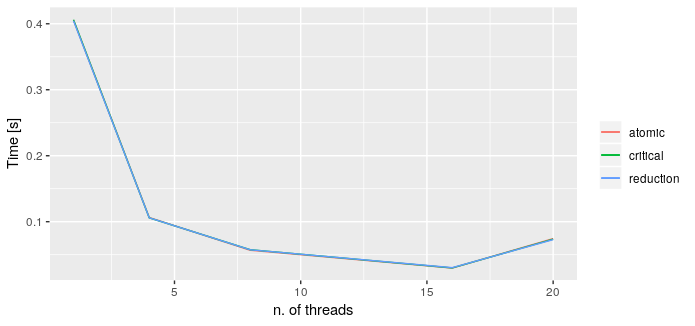
\includegraphics[scale=.8]{correct_final}
		\caption{Comparison between parallel implementations}
		\label{fig_1}
	\end{centering}
\end{figure}

\begin{figure}[h!]
	\begin{centering}
		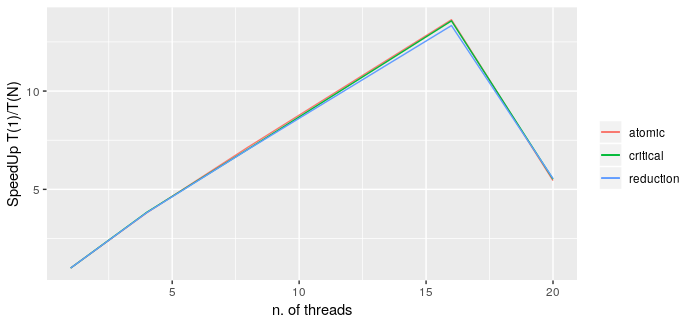
\includegraphics[scale=.8]{speedup}
		\caption{Comparison between parallel implementations(2)}
		\label{fig_2}
	\end{centering}
\end{figure}
\end{document}          
